\documentclass[]{article}

\usepackage{graphicx}
\usepackage{amssymb}
\usepackage{amsthm}
\usepackage{amsmath}
\usepackage{multirow}
\usepackage[section]{placeins}
\usepackage{listings}
\usepackage{hyperref}
\hypersetup{
	colorlinks,
	citecolor=black
	filecolor=black,
	linkcolor=blue,
	urlcolor=black
}
\lstset{
	language=MATLAB,
	basicstyle=\scriptsize\sffamily,
	numbers=left,
	numberstyle=\tiny,
	frame=tb,
	columns=fullflexible,
	showstringspaces=false
}

%opening
\title{EML6934 Optimal Control \\ Final Project}
\author{Elias Reyes}

\begin{document}
	
	\maketitle
	\thispagestyle{empty}
	\newpage
	\pagenumbering{roman}
	\newpage
	\tableofcontents
	\newpage
	\listoffigures
	\listoftables
	\newpage
	\lstlistoflistings
	\newpage
	\pagenumbering{arabic}
	
	\section{Problem Statement}
	\section{Differential Equations of Motion}
	The equations of motion were derived using both Newton's second law and Lagrange's equations. The schematic for the problem can be seen Figure \ref{fig:schematic}. The spacecraft is modeled as point \(P\) of  mass \(m\). The spacecraft moves relative to an inertial reference frame \(l\). The reference frame fixed in \(l\) is expressed as \(\{e_{x},e_{y},e_{z}\}\). The position of the spacecraft is denoted as \(r_{P/O}\), where \(O\) is modeled as the sun, fixed in \(l\). The spacecraft is parameterized in the basis \(\{u_{r},u_{\theta},u_{z}\}\), where the rotation is about \(u_{z}\) = \(e_{z}\). The rotation creates an angle \(\theta\) between \(e_{x}\) and \(u_{r}\), which can be seen in Figure \ref{fig:rotation2}.
	\begin{figure}
		\centering
		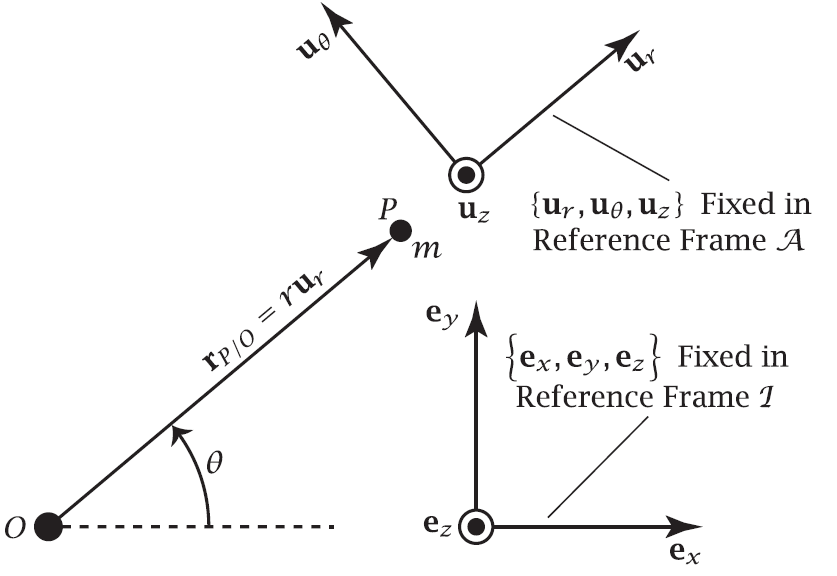
\includegraphics[width=85mm,scale=0.85]{midterm_schematic.png}
		\caption{Schematic of particle moving in an inertially fixed plane}
		\label{fig:schematic}
	\end{figure}
	\begin{figure}
		\centering
		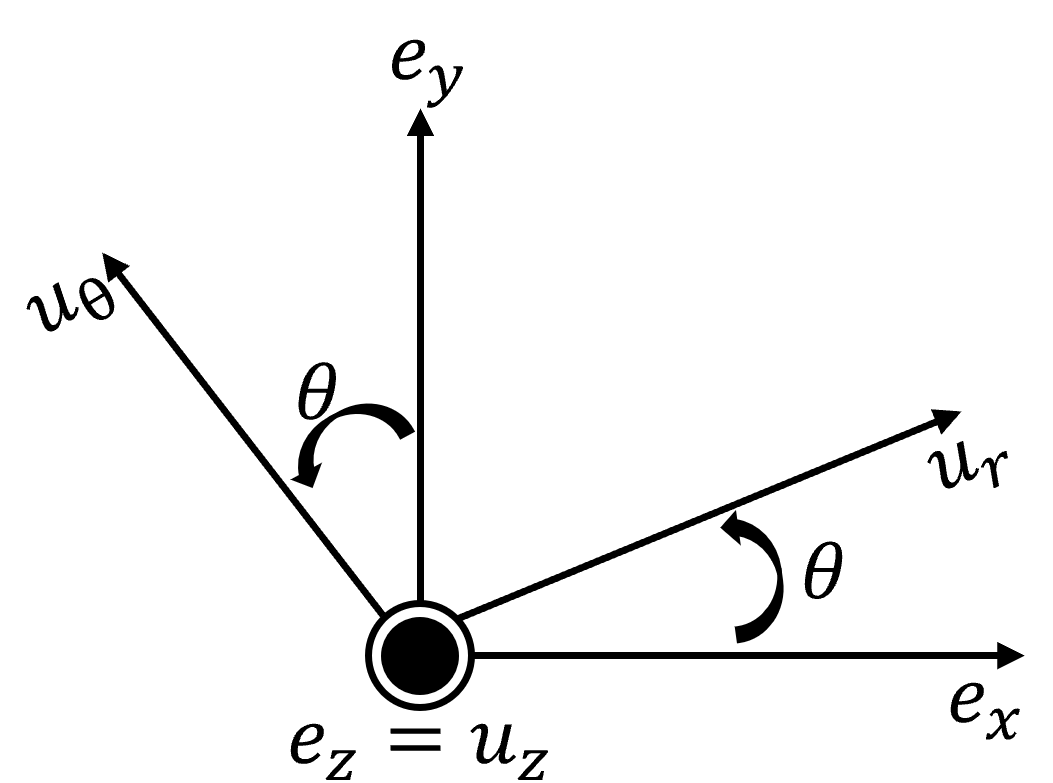
\includegraphics[width=75mm,scale=0.75]{rotation.png}
		\caption{Reference frame rotation}
		\label{fig:rotation2}
	\end{figure}
	\noindent 
	Two forces are said to act on the spacecraft. The first is the gravitational force which is given as
	\begin{equation} \label{grav_force}
		G = -m\mu\frac{r_{P/O}}{||r_{P/O}||^3},
	\end{equation}
	%\[G = -m\mu\frac{r_{P/O}}{||r_{P/O}||^3},\]
	while the second is the thrust force given as\\
	\begin{equation} \label{thrust_force}
		T = Tw,
	\end{equation}
	%\[T = Tw,\]
	where \(w\) is the unit vector that lies an angle \(\beta\) from the direction \(u_{\theta}\) as seen in Figure \ref{fig:beta}.
	\begin{figure}
		\centering
		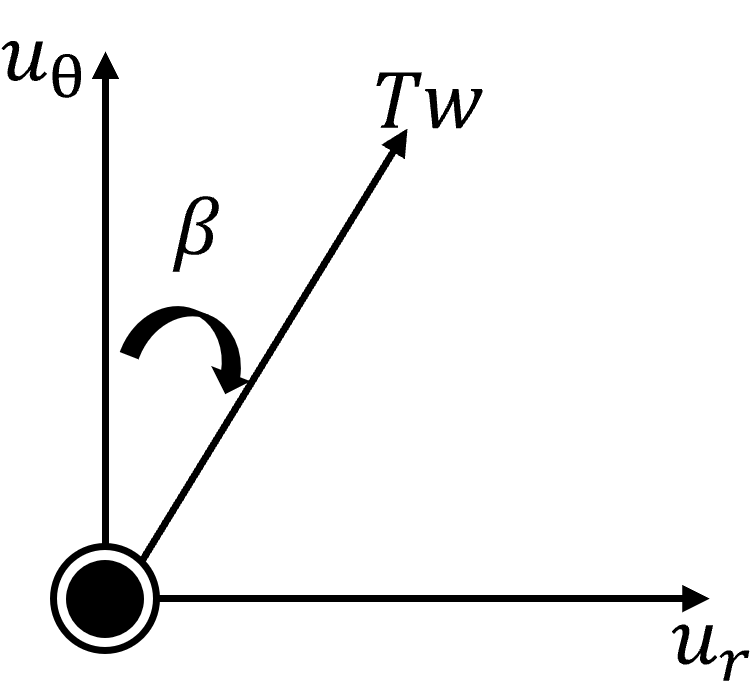
\includegraphics[width=50mm,scale=0.5]{beta.png}
		\caption{Thrust Force at Angle \(\beta\)}
		\label{fig:beta}
	\end{figure}
	\subsection{Position, Velocity and Acceleration of the Spacecraft}
	As seen in Figure \ref{fig:schematic}, the position of the spacecraft represented in reference frame \(A\), is given as 
	\begin{equation} \label{position}
		^A\vec{r}_{P/O} = ru_{r}.
	\end{equation}
	The velocity can then be represented in the inertial frame \(l\) by using equation \ref{golden_rule}, where \(^l\vec{\omega}^A\) is the angular velocity between reference frame \(l\) and \(A\).
	\begin{equation} \label{golden_rule}
		\frac{^ld\vec{r}_{P/O}}{dt} = \frac{^Ad\vec{r}_{P/O}}{dt} +\ ^l\vec{\omega}^A\  \times\  ^A\vec{r}_{P/O} 
	\end{equation}
	Using Equation \ref{golden_rule}, the velocity of the spacecraft in the inertial frame is then formulated as
	\begin{align}
		^l\vec{v_{p}} &= \frac{^ld\vec{r}_{P/O}}{dt} \nonumber\\
		^l\vec{v_{p}} &= \dot{r}u_{r} +\ \dot{\theta}u_{z}\ \times\ ru_{r} \nonumber\\
		^l\vec{v_{p}} &= \dot{r}u_{r} +\ \dot{\theta}ru_{\theta} \label{velocity}
	\end{align}
	The acceleration of the particle can then be formulated as 
	\begin{align}
		^l\vec{a_{p}} &= \frac{^ld\vec{v_{P}}}{dt} \nonumber\\
		^l\vec{a_{p}} &= \frac{^Ad\vec{v_{P}}}{dt} +\ ^l\vec{\omega}^A\  \times\  ^A\vec{v_{P}} \nonumber\\
		^l\vec{a_{p}} &= \ddot{r}u_{r} +\ (\ddot{\theta}r+\dot{\theta}\dot{r})u_{\theta} +\ \dot{\theta}\dot{r}u_{\theta} -\ \dot{\theta}^2ru_{r} \nonumber\\
		^l\vec{a_{p}} &= (\ddot{r} -\ \dot{\theta}^2r)u_{r} +\ (\ddot{\theta}r+2\dot{\theta}\dot{r})u_{\theta}   \label{acceleration}
	\end{align}
	%\[^A\vec{r}_{P/O}\]
	
	%\figurename{Schematic of a particle in a an inertially fixed plane.}
	\subsection{Newton's Second Law for A Particle}
	The equations of motion are first derived using Newton's Second Law for a Particle. Newton's Second Law for a particle is represented by
	\begin{align}
		\sum{F_{P}} = m_{P} * a_{P}. \label{newton}
	\end{align}
	\vspace{2mm}\newline
	Figure \ref{fig:FBD} represents the free body diagram of the particle system. \(F_{G}\), represented by equation \ref{grav_force}, is the gravitational force and acts along the \(u_{r}\) direction. \(F_{T}\), represented by equation \ref{thrust_force}, is the thrust force and acts in the direction \(w\). It can be seen in Figure \ref{fig:beta} that the thrust force can be re-written as 
	\begin{align}
		F_{T} = Tsin(\beta)u_{r} + T\cos(\beta)u_{\theta}, \label{F_T}
	\end{align}
	while the gravitational force can be written as
	\begin{align}
		F_{G} = -m\mu\frac{1}{r^2}u_{r}. \label{F_G}
	\end{align}
	We can now substitute equations \ref{acceleration},  \ref{F_T}, and \ref{F_G} into equation \ref{newton} to obtain
	\begin{align*}
		-m\mu\frac{1}{r^2}u_{r} + Tsin(\beta)u_{r} + T\cos(\beta)u_{\theta} = m[(\ddot{r} -\ \dot{\theta}^2r)u_{r} +\ (\ddot{\theta}r+2\dot{\theta}\dot{r})u_{\theta}]. 
	\end{align*}
	After equating terms, the two equations of motion using Newtons Seconds become:
	\begin{align}
		(u_{r})\qquad      &  \ddot{r}      = \dot{\theta}^2r - \frac{\mu}{r^2} + \frac{Tsin(\beta)}{m} \label{eom1}\\
		(u_{\theta})\qquad &  \ddot{\theta} = -\frac{2\dot{r}\dot{\theta}}{r}   + \frac{T\cos(\beta)}{mr} \label{eom2}
	\end{align}
	\begin{figure}
		%	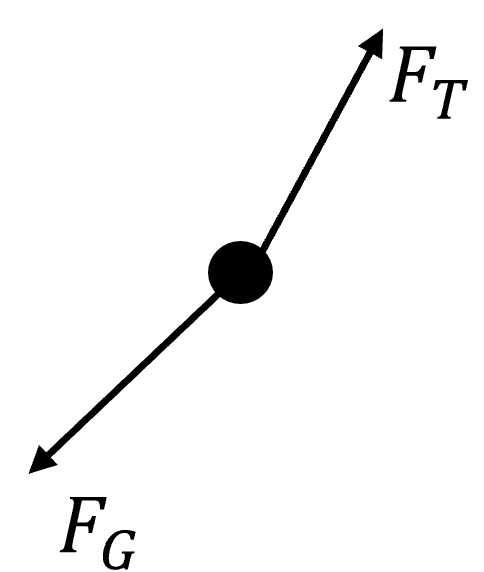
\includegraphics[width=\linewidth]{FBD.png}
		\centering
		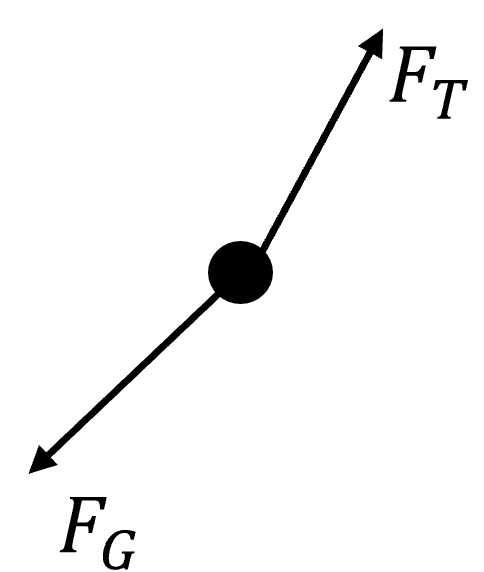
\includegraphics[width=50mm,scale=0.5]{FBD.png}
		\caption{Free Body Diagram}
		\label{fig:FBD}
	\end{figure}

\end{document}
